\documentclass[11pt]{article}

% --- layout ---
\usepackage[a4paper,margin=1in]{geometry}
\usepackage{microtype}
\usepackage{lmodern}

% --- graphics & tables ---
\usepackage{graphicx}
\graphicspath{{figures/}}
\usepackage{booktabs}

% --- math ---
\usepackage{amsmath,amssymb}

% --- references (numeric, arXiv-style; [1-3,6] range compression) ---
\usepackage[numbers,sort&compress]{natbib}
% Clickable but ink-black links (no blue) --- standard for preprints.
\usepackage[colorlinks=true,allcolors=black]{hyperref}

% --- convenience macros ---
\newcommand{\curia}{CURIA}
\newcommand{\rinalmo}{RiNALMo}
\newcommand{\rnafm}{RNA-FM}
\newcommand{\toga}{TOGA}

\title{Cross-species ncRNA annotation using synteny-constrained embedding similarity}
\author{Bogdan M. Kirilenko\\\small Independent Researcher}
\date{\today}

\begin{document}

\maketitle

\begin{abstract}
Reference-based annotation transfer via orthology has been highly successful for
protein-coding genes but remains challenging for non-coding RNAs (ncRNAs) due to
weak sequence conservation, ambiguous transcript boundaries, and incomplete
annotations. Here we present \curia{}, a pipeline for cross-species ncRNA
annotation that combines genome alignment chains with embedding-based
representations derived from RNA foundation models. \curia{} formulates
cross-species ncRNA correspondence as synteny-constrained matching in embedding
space. It first identifies candidate loci using a simplified TOGA-based
projection, then detects localized subregions (``islands'') within transcripts,
and finally establishes cross-species correspondence using similarity of
embedding representations. Because the embedding model is largely stable
across sequence context, each island is embedded once and matched at nucleotide
resolution. Using a conservative annotation-based evaluation across 19
mammalian genomes, \curia{} identified short ncRNA loci; in the human-to-mouse
comparison, 52.4\% of predicted loci overlapped an annotated exon (any overlap).
It further uncovered ${\sim}230$ candidate intergenic loci potentially
corresponding to conserved ncRNA elements absent from current annotations. These
results suggest that combining synteny with embedding-based similarity can
complement conventional sequence conservation for cross-species ncRNA annotation
in settings characterized by weak or heterogeneous primary-sequence conservation,
establishing a proof of concept for integrating comparative genomics with RNA
foundation-model embeddings for genome-scale ncRNA analysis.
\end{abstract}

\section{Introduction}
\label{sec:intro}

\subsection{Protein-coding orthology as a tractable problem}
Orthology inference for protein-coding genes is well established and supported by
scalable annotation transfer pipelines
\citep{kirilenkoIntegratingGeneAnnotation2023,sharmaIncreasedAlignmentSensitivity2017,kentEvolutionsCauldronDuplication2003,sharmaCESAR20Substantially2017,herreroEnsemblComparativeGenomics2016,fitchDistinguishingHomologousAnalogous1970,kooninOrthologsParalogsEvolutionary2005}.
Strong sequence conservation, together with constraints imposed by open reading
frames, enables reliable cross-species mapping of gene loci
\citep{sharmaIncreasedAlignmentSensitivity2017,sharmaCESAR20Substantially2017}.
Methods such as TOGA, which combine genome alignment chains with coding sequence
structure, achieve high accuracy at genome scale. However, these approaches rely
on properties specific to protein-coding genes and do not generalize to
non-coding RNAs. In particular, they assume conserved coding structure and
detectable sequence similarity, which are often absent outside protein-coding
contexts.

In this work, we do not attempt to infer evolutionary orthology. Instead, we
identify candidate cross-species correspondences supported by genomic synteny
and embedding similarity, and frame the task as synteny-constrained annotation
transfer.

\subsection{The ncRNA orthology challenge}
Cross-species correspondence is difficult to establish for ncRNAs because the
relevant conserved unit is often unclear. For many ncRNAs, evolutionary
conservation is less readily captured by primary-sequence identity than for
protein-coding genes: related RNAs may retain similar molecular functions,
structural features, or localized conserved elements despite substantial
sequence divergence
\citep{ulitskyLincRNAsGenomicsEvolution2013,
  diederichsFourDimensionsNoncoding2014,
  hezroniPrinciplesLongNoncoding2015,
  rivasEvolutionaryConservationRNA2021,
  ulitskyEvolutionRescueUsing2016,
  statelloGeneRegulationLong2021}.
Conservation may also be restricted to short motifs or local domains rather than
extending across the complete transcript. At the same time, transcript
boundaries and isoform structures are frequently ambiguous, and ncRNA
annotations remain incomplete and heterogeneous across species
\citep{mattickLongNoncodingRNAs2023,perteaCHESSNewHuman2018}.
Together, these properties complicate both annotation transfer and its
evaluation.

These problems are especially acute for lncRNAs. Annotated loci may span tens of
kilobases and contain localized candidate domains separated by long intervening
sequence. Whole-locus comparison can therefore dilute localized correspondence,
and complete loci may exceed the input length supported by current RNA
foundation models. This motivates searching for candidate conserved subregions
rather than requiring end-to-end transcript correspondence.

\subsection{Limitations of existing approaches}

Existing methods address several related tasks, but none directly combines
reference-guided annotation transfer with localization and comparison of
candidate ncRNA subregions within syntenic genomic loci.

Covariance-model approaches implemented in Infernal and distributed through
Rfam can sensitively identify members of established RNA families
\citep{nawrockiInfernal11100fold2013,
  ontiveros-palaciosRfam15RNA2025}. Their application, however, depends on a
predefined family alignment and consensus sequence--structure model. They are
therefore well suited to annotating known RNA families, but less applicable to
reference loci for which no curated family model exists.

Structure-aware alignment methods such as LocARNA and RNAforester compare
supplied RNA sequences using explicit sequence--structure models
\citep{willLocARNA20Versatile2024,hochsmannLocalSimilarityRNA2003}. These methods
address the comparison of already defined RNA intervals, rather than locating a
corresponding element within a genome-scale syntenic search region.

Comparative screening methods such as RNAz and EvoFold identify genomic regions
with evidence of evolutionarily conserved RNA secondary structure in multiple
sequence alignments
\citep{gruberRNAz20Improved2010,pedersenIdentificationClassificationConserved2006}. Their objective is de novo
discovery of candidate structured RNA elements, rather than transfer of a
specific reference annotation to a query genome. They also depend on detectable
comparative sequence and structural signals within the input alignment.

CURIA addresses a different task. Starting from a reference ncRNA annotation and
pairwise genome alignment chains, it first restricts the search to candidate
syntenic loci and then localizes and ranks corresponding subregions using learned
RNA representations. This formulation does not require a pre-existing RNA family
model, a supplied query transcript, or end-to-end conservation of the annotated
reference locus.

\subsection{Synteny-constrained embedding matching}

An underexplored strategy is to use pretrained RNA-language-model
representations as a localized similarity signal within syntenically constrained
genomic search regions. Genome alignment chains provide candidate regions that
preserve genomic context and therefore indicate where a corresponding ncRNA may
be sought
\citep{zoonomiaconsortiumComparativeGenomicsMultitool2020,
  armstrongProgressiveCactusMultiplegenome2020}.
RNA foundation models such as RNA-FM
\citep{chenInterpretableRNAFoundation2022}, RiNALMo
\citep{penicRiNALMoGeneralpurposeRNA2025}, and related approaches such as RNABERT
\citep{akiyamaInformativeRNABase2022} provide learned representations associated
with RNA family identity, secondary-structure-related properties, and downstream
predictive tasks
\citep{vahabAdvancingNoncodingRNA2025}.
Applying these models as unconstrained genome-wide scanners would be
computationally impractical, whereas restricting comparison to chain-defined
candidate loci makes localized RNA-specific matching feasible. This combination
supports comparison of ncRNA loci in settings where primary-sequence conservation
is weak or heterogeneous.

\begin{figure}[t]
  \centering
  % Generated by analysis/make_figures.py (fig1_embeddings) from RiNALMo
  % embeddings cached in analysis/data/fig1_embeddings.npz.
  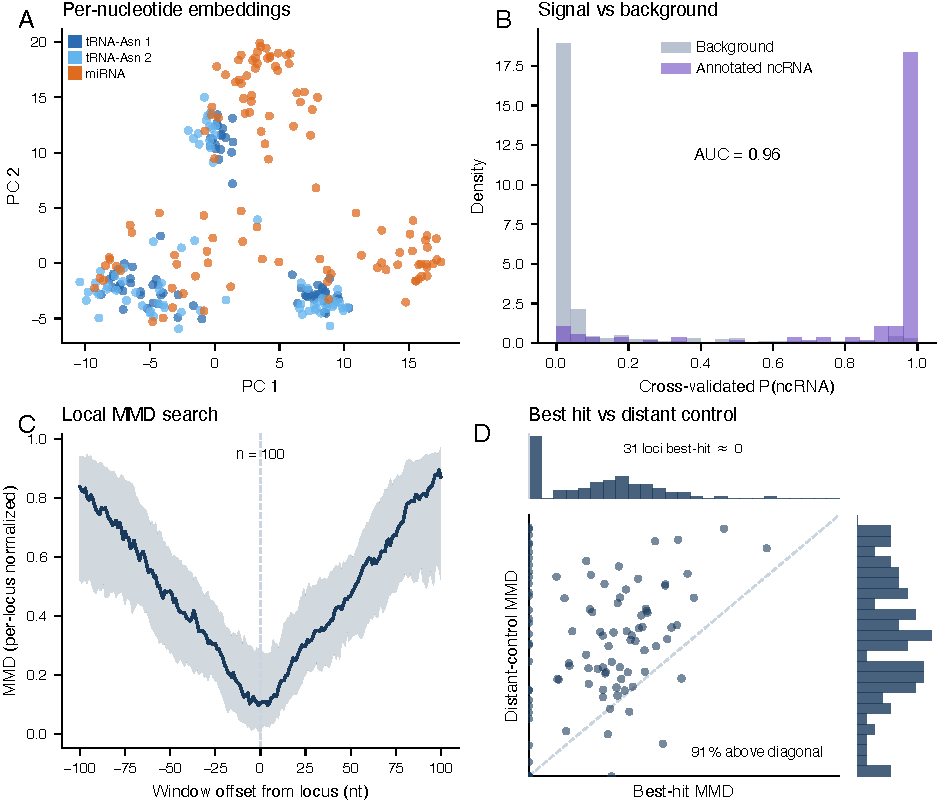
\includegraphics[width=\linewidth]{fig1_embeddings.pdf}
  \caption{Illustrative embedding behavior supporting local ncRNA comparison.
  \textbf{(A)} Per-nucleotide embeddings
  (matching PCA, first two components) for two human tRNA-Asn-GTT gene copies
  (\textit{tRNA-Asn-GTT-chr1-139} and \textit{-140}, $74$\,nt each) and one
  pre-miRNA (\textit{MIR103A1}, ENST00000362168, $110$\,nt), all from the human
  genome assembly hg38; each point is a nucleotide. The tRNA copies cluster
  together while the miRNA forms a distinct cluster. \textbf{(B)} Out-of-fold
  probability from a 5-fold cross-validated logistic classifier trained on the
  embeddings to distinguish annotated hg38 ncRNAs (purple; tRNA, snoRNA, miRNA)
  from background sequences (gray; intergenic and dinucleotide-shuffled): ncRNAs
  score near $1$ and background near $0$ (AUC ${\approx}0.96$), showing the
  embeddings separate the selected RNA-derived sequences from genomic background.
  Panel (B), titled ``Illustrative embedding separability'' within the figure, is
  an illustrative separability experiment on a small balanced set and is not the
  production island detector used in the pipeline (Section~\ref{sec:refisland}),
  which is trained on a different biotype set and negatives and operates at a
  different threshold.
  \textbf{(C)} Maximum Mean Discrepancy (MMD) between a short-ncRNA reference and
  windows tiled across its extended locus, versus offset from the annotated
  position (median and interquartile range over $n=100$ short ncRNAs, each locus
  min--max normalized). MMD is minimised at the true position (offset $0$) and
  rises with positional shift. \textbf{(D)} Best-hit MMD versus a distant control
  window ($250$\,nt away) for the same $n=100$ loci, with marginal histograms.
  Best-hit MMD concentrates near $0$ (31 loci essentially perfect), whereas the
  distant control almost never does; 91\% of loci lie above the diagonal
  (matched window more similar than the control).}
  \label{fig:embeddings}
\end{figure}

\subsection{Method overview}

We formulate cross-species ncRNA correspondence as the matching of
embedding-supported regions within loci defined by genome alignment chains.
Candidate loci are first identified using a chain-based projection adapted from
principles used in TOGA. The projection uses alignment coverage across exonic,
intronic, and flanking sequence to provide locus-level syntenic context that is
not determined solely by conservation within the ncRNA itself
\citep{kirilenkoIntegratingGeneAnnotation2023,
  sharmaIncreasedAlignmentSensitivity2017}.

Within each candidate locus, \curia{} compares RNA-language-model
representations using one of two geometry-dependent branches. Compact,
single-exon ncRNAs are compared as complete regions using Maximum Mean
Discrepancy (MMD)
\citep{grettonKernelTwoSampleTest2012}, which measures the difference between
the distributions of their per-position embedding vectors. Longer or
multi-exon loci are processed by a localized-subregion workflow, in which
detector-positive subregions are matched by Smith--Waterman local alignment
\citep{smithIdentificationCommonMolecular1981} over a per-token cosine-similarity
matrix. Both branches provide continuous scores for ranking candidate
correspondences without requiring nucleotide sequence alignment.

\subsection{Contributions}
In this work, we:
\begin{enumerate}
  \item Formulate cross-species ncRNA annotation as synteny-constrained matching
  in RNA embedding space.
  \item Introduce \curia{}, a pipeline that combines chain-based locus projection
  with localized embedding-based comparison.
  \item Develop complementary strategies for compact and extended ncRNA loci,
  including boundary refinement for short ncRNAs and localized subregion
  matching for longer or multi-exon loci.
  \item Demonstrate the approach at genome scale across 19 mammalian genomes and
  identify recurrent candidate correspondences that are not fully explained
  by conventional sequence-similarity measures.
\end{enumerate}

\section{Methods}
\label{sec:methods}

% =====================================================================
% This section was rewritten for the RiNALMo pipeline. Parameter values
% are taken from the current code:
%   modules/model_registry.py
%   modules/pipeline/short_ncrna.py
%   modules/pipeline/matchers/rinalmo.py
%   modules/logreg_signal_noise/build_rinalmo_finding.py
% =====================================================================

\subsection{Pipeline overview}

\curia{} is a computational pipeline for genome-scale cross-species ncRNA
correspondence that combines chain-guided locus prediction with embedding-based
comparison (Figure~\ref{fig:pipeline}). Given a reference genome with ncRNA
annotations, a query genome, and pairwise genome alignment chains, \curia{}
produces refined query loci for compact single-exon ncRNAs and scored
reference--query subregion correspondences for longer or multi-exon loci.

The pipeline consists of seven stages:
\begin{enumerate}
    \item \textbf{Preprocessing.} Isoforms assigned to the same locus and strand are
    merged into a \emph{union exon model} by taking the union of their exonic
    intervals in genomic order.

    \item \textbf{Candidate region prediction.} Genome alignment chains are used to
    identify candidate query regions with a chain-based classifier adapted from
    principles used in TOGA
    (Section~\ref{sec:candidate}).

    \item \textbf{Short ncRNA refinement.} For compact single-exon ncRNAs, the
    projected candidate locus is refined by an embedding-based local boundary
    search, without decomposition into subregions
    (Section~\ref{sec:short}).

    \item \textbf{Reference subregion detection.} For longer or multi-exon loci,
    localized embedding-supported subregions (``islands'') are identified in the
    reference locus
    (Section~\ref{sec:refisland}).

    \item \textbf{Chain-guided subregion projection.} Each reference island is
    projected through the genome alignment chain to define a corresponding search
    region in the query genome
    (Section~\ref{sec:projisland}).

    \item \textbf{Query subregion detection.} Candidate query islands are identified
    within the projected search regions associated with the reference islands
    (Section~\ref{sec:queryisland}).

    \item \textbf{Reference--query subregion matching.} Reference and query islands
    are compared by embedding-based local matching, producing scored
    reference--query subregion correspondences
    (Section~\ref{sec:islandalign}).
\end{enumerate}

\textbf{Branch routing.} Loci are assigned to processing branches according to
the geometry of their union exon models rather than their annotation biotypes,
because biotype labels do not reliably determine whether a locus is best treated
as a compact complete region or as a set of localized subregions. Some annotated
lncRNAs are short and single-exonic, whereas some compact ncRNA classes are
multi-exonic.

Single-exon loci of length $\leq 256$\,nt are processed as complete loci.
Single-exon loci of length $257$--$320$\,nt are represented as a single
whole-exon island. Single-exon loci longer than $320$\,nt and all multi-exon loci
are scanned for detector-positive islands
(Section~\ref{sec:refisland}). These categories form a partition, and each locus
is processed exactly once.

The union exon model is a locus-level search representation rather than a
reconstructed mature transcript. Because exons are unioned across isoforms, the
model may combine segments that do not coexist in any single transcript. It is
used only to define the search space for localized signal.

\begin{figure}[t]
  \centering
  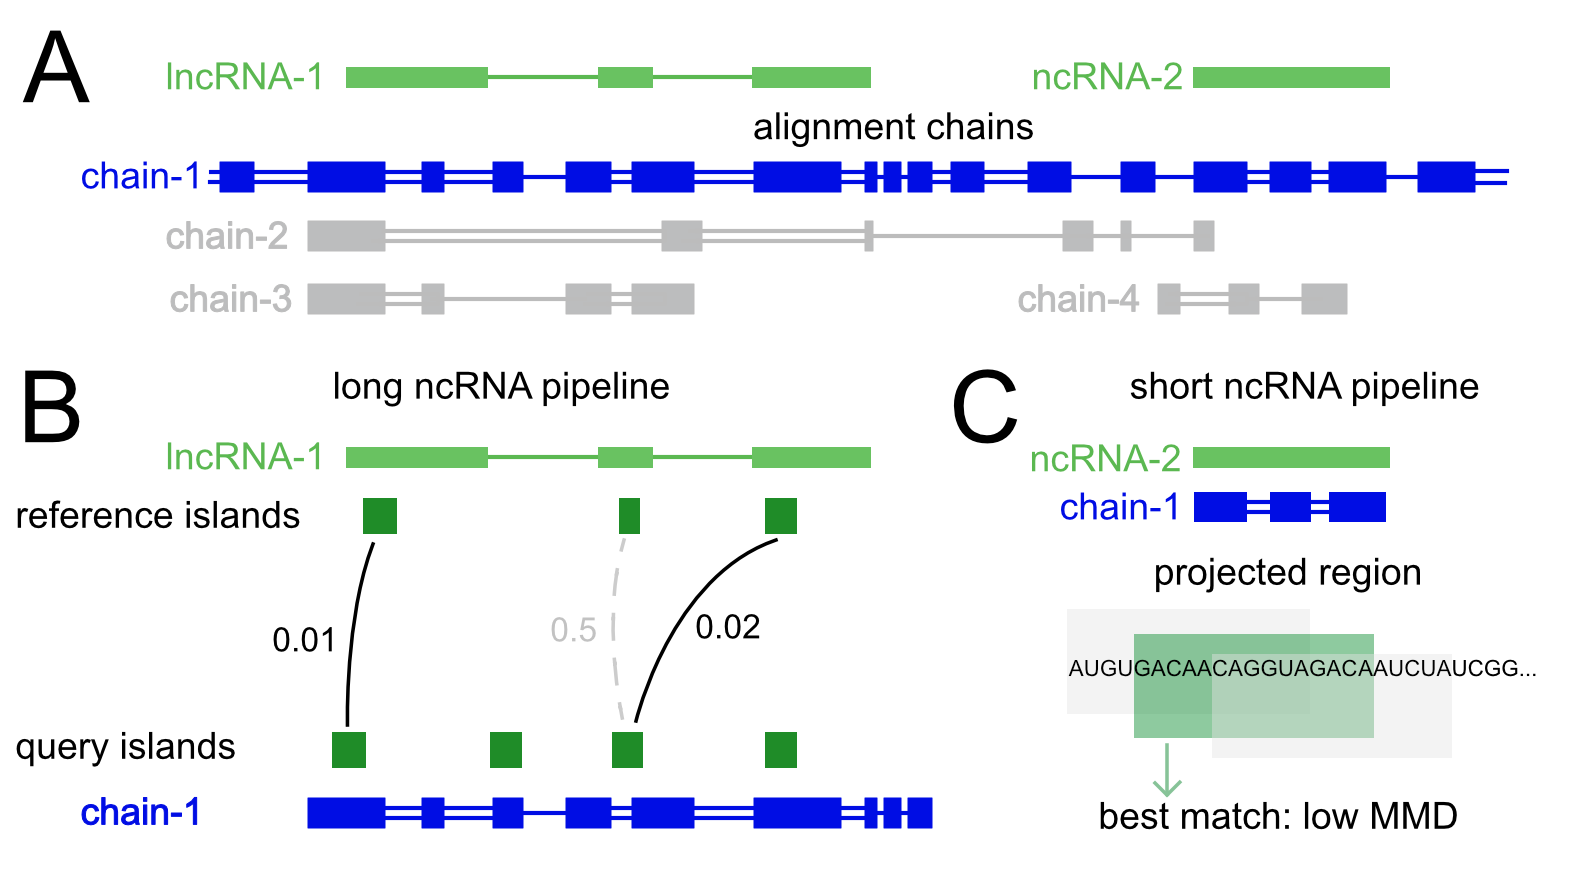
\includegraphics[width=\linewidth]{fig2_pipeline.png}
  \caption{Overview of the \curia{} pipeline for cross-species ncRNA
  correspondence analysis. \textbf{(A)} Genome alignment chains restrict the
  search space by defining candidate loci between reference and query genomes.
  \textbf{(B)} For island-branch loci, localized subregions (``islands'') are detected
  and matched across species using embedding-based similarity, enabling
  localization of candidate corresponding regions within transcripts. \textbf{(C)}
  For short ncRNAs, correspondence is resolved via local boundary refinement using
  sliding-window matching in embedding space.}
  \label{fig:pipeline}
\end{figure}

\subsection{Input data}
\curia{} requires three types of input data:
\begin{enumerate}
    \item \textbf{Reference genome and annotation.} The reference genome is provided
    in 2bit format, with ncRNA annotations in BED12 format including
    \texttt{transcript\_id}, \texttt{gene\_id}, and \texttt{biotype}.
    Protein-coding transcripts are used during candidate-region prediction to
    compute synteny-related features but are excluded from downstream ncRNA
    analysis.
    \item \textbf{Query genome.} The query genome is provided in 2bit format.
    Query-side annotations are not required for prediction but may be used
    for evaluation.
    \item \textbf{Genome alignment chains.} Pairwise reference--query genome
    alignments are provided in UCSC chain format and define the search space
    used for locus projection. Low-scoring chains are filtered during loading.
\end{enumerate}

\subsection{Candidate region prediction}
\label{sec:candidate}

\textbf{Input.} Union exon models and genome alignment chains.

\textbf{Operation.} \curia{} uses a chain-based locus-projection procedure
adapted from the orthology-classification framework used in TOGA
\citep{kirilenkoIntegratingGeneAnnotation2023} to define coarse candidate regions
in the query genome rather than reconstruct complete transcripts
(Figure~\ref{fig:pipeline}A).

For each chain--locus pair, seven features describing chain coverage and reference
exon geometry are computed: log-transformed synteny gene count
(\texttt{synteny\_log1p}), global exonic occupancy
(\texttt{gl\_exo}), $\pm10$\,kb flank coverage
(\texttt{flank\_cov}), exonic-length-to-query-span ratio
(\texttt{exlen\_to\_qlen}), exonic fraction
(\texttt{exon\_perc}), exon count
(\texttt{ex\_num}), and a single-exon indicator
(\texttt{single\_exon}).

A gradient-boosted decision-tree classifier, trained on labeled human--mouse
chain--transcript pairs, assigns a correspondence probability to each pair.
Pairs with predicted probability at least 0.5 are retained. For loci annotated
as lncRNA, a relaxed threshold of 0.3 is used to favor candidate-region recall.
These biotype-dependent thresholds are applied before the subsequent
geometry-based branch routing.

For query genomes in which the classifier is overly conservative, candidate
regions may instead be seeded from the highest-scoring alignment chain for each
reference locus, irrespective of the classifier call.

For each retained chain--locus pair, the reference locus is projected through
the corresponding alignment chain. The candidate query interval is defined by
the span of chain blocks overlapping the reference locus and is extended by
flanking sequence to accommodate local projection uncertainty. If multiple chains
pass the selection criterion for the same reference locus, all corresponding
candidate intervals are retained.

\textbf{Output.} Projected candidate query regions with their associated
reference loci, chains, and classifier metadata.

\textbf{Rationale.} Downstream embedding-based comparison requires only a coarse
locus-level search space. This avoids imposing coding-sequence constraints or
attempting to reconstruct complete query transcripts.

\subsubsection{Classifier training and evaluation partitioning}
\label{sec:classifier-training}

Chain--transcript pairs are labeled using the TOGA orthology-classification
procedure on which this step is based
\citep{kirilenkoIntegratingGeneAnnotation2023}. Pairs assigned to the ORTH
category form the positive class, whereas pairs assigned to the PARA category
form the negative class; all other categories are excluded from training. These
labels are used only to train the chain-based candidate-region classifier and
should not be interpreted as ncRNA orthology assignments produced by \curia{}.

The seven classifier features describe chain geometry and reference-side exon
structure: synteny coverage, gene-level exonic overlap, flank coverage,
exon-to-query-length ratio, exon fraction, exon count, and a single-exon
indicator. Neither RNA embeddings nor query-side ncRNA annotations are used.

A gradient-boosted decision-tree classifier is trained on a balanced sample of up
to 20{,}000 pairs per class. Model development uses a fixed random 75/25
stratified train/test split, and performance is summarized by five-fold
stratified cross-validated AUC. Splits are stratified by class label but are not
grouped by transcript, gene, locus, chromosome, or family. Related or neighboring
loci may therefore occur in different folds, and the reported AUC should be
interpreted as a measure of ORTH--PARA feature separability rather than as a
strict held-out-locus generalization estimate.

The classifier is used only to define the candidate search space; downstream
embedding-based matching and annotation-based evaluation are performed
independently of its training labels.

\subsection{RNA embeddings}
\label{sec:embeddings}

Sequences are represented by per-nucleotide embeddings from the RiNALMo
general-purpose RNA foundation model
(\texttt{giga-v1}; 650M parameters, 1280-dimensional per-token embeddings)
\citep{penicRiNALMoGeneralpurposeRNA2025}.

Two task-specific linear projections are used. A $k{=}16$ PCA, fitted on
10{,}368 per-token embeddings, is applied for position-level matching. A
$k{=}64$ PCA, fitted on the 18{,}827 mean-pooled training windows described
below, is applied for localized subregion detection.

The corresponding PCA transformations, the compact-ncRNA-versus-background
detector, scan and match thresholds, and embedding settings are stored as
versioned pipeline artifacts and selected through a model registry.

\subsection{Short ncRNA pipeline}
\label{sec:short}

Compact single-exon ncRNA loci can be compared directly without decomposition
into localized subregions (Figure~\ref{fig:pipeline}C). This branch processes all
single-exon loci of length up to 256\,nt, irrespective of annotation biotype;
typical examples include miRNAs, tRNAs, snoRNAs, and snRNAs, although short
single-exon loci annotated as lncRNA may also enter this branch.

For each locus, the reference sequence is embedded, and the corresponding query
region is symmetrically extended, when necessary, to provide a search span of
1.1 times the reference length. Candidate windows matching the reference length
are tiled across the query region and compared with the reference using MMD
(Section~\ref{sec:mmd}). The best-scoring window is then refined by local boundary
perturbation of up to $\pm 5$\,nt, subject to a final length constraint of
$0.8$--$1.2\times$ the reference length. Before comparison, embeddings are
projected from 1280 to 16 dimensions using the matching PCA.

\textbf{Output.} Refined query coordinates with an MMD-based similarity score.

\subsection{Similarity in embedding space (MMD)}
\label{sec:mmd}

For short ncRNAs, window similarity is quantified using Maximum Mean Discrepancy
(MMD) \citep{grettonKernelTwoSampleTest2012} with an RBF kernel, treating
per-position embeddings as empirical distributions:
\begin{equation}
    \widehat{\mathrm{MMD}}_u^2(X, Y) =
    \frac{1}{n(n-1)}\sum_{i \neq j} k(x_i, x_j)
    + \frac{1}{m(m-1)}\sum_{i \neq j} k(y_i, y_j)
    - \frac{2}{nm}\sum_{i,j} k(x_i, y_j),
\end{equation}
where $k(x, y) = \exp(-\gamma \lVert x - y \rVert^2)$ and
$X = \{x_1, \dots, x_n\}$ and $Y = \{y_1, \dots, y_m\}$ are the sets of
per-position embedding vectors for the two sequence windows. This is the
unbiased empirical estimator, with self-terms excluded from the within-sample
sums.

The implementation reports
$\sqrt{\max(\widehat{\mathrm{MMD}}_u^2, 0)}$, because the unbiased finite-sample
estimate may be negative. A reported value of zero may therefore result from
clipping and does not necessarily indicate identical empirical distributions.
Lower MMD values indicate more similar embedding distributions.

The kernel bandwidth $\gamma$ is determined separately for each reference locus
using the median pairwise-distance heuristic on its per-position embeddings and
is then held fixed for all query-window comparisons at that locus. The resulting
scores are suitable for ranking candidate windows within a locus, but are not
globally calibrated across loci or biotypes. Cross-locus comparisons and global
thresholds should therefore be interpreted approximately.

\subsection{Reference island detection}
\label{sec:refisland}

To identify localized embedding patterns associated with annotated compact
ncRNAs, we trained a logistic regression classifier on fixed-length genomic
sequence windows represented in RiNALMo embedding space. Positive loci were
sampled from annotated miRNAs, snoRNAs, snRNAs, scaRNAs, and
\texttt{misc\_RNAs}; lncRNAs were excluded from detector training.

For each selected single-exon ncRNA locus, the gene body together with
150\,nt of flanking sequence on each side was divided into 128-nt windows with
a stride of 24\,nt. A window was labeled positive when it overlapped the
annotated ncRNA by at least 20\,nt. Other windows from the same region were
labeled negative. Additional negative examples were generated by sampling N-free genomic regions
of comparable length from the primary chromosomes and tiling them using the same
window and stride.

Each window was embedded with RiNALMo, mean-pooled across positions, and
projected from 1280 to 64 dimensions using the detection PCA before classifier
training. Training loci were balanced across biotypes, with up to 150 loci per
biotype and an additional 71 held-out loci per biotype used for threshold
calibration. The committed training cache contains 18{,}827 windows:
6{,}538 positive and 12{,}289 negative. In five-fold cross-validation, the
classifier achieved ROC-AUC $\approx 0.79$. At a threshold calibrated to a
background false-positive rate of at most 20\%, it detected approximately 78\%
of windows overlapping an annotated element by at least 40\,nt.

The detector therefore distinguishes embedding patterns associated with the
compact ncRNA classes represented in its positive training set from the sampled
genomic background. Contiguous detector-positive regions are termed
``islands.'' This is an operational definition: detector positivity does not
establish stable RNA structure, biological function, or membership in a general
ncRNA class.

For reference-locus analysis, the concatenated exonic sequence of each union
exon model is scanned using a 128-nt sliding window with a stride of 40\,nt.
Windows are embedded, mean-pooled, projected into the detection PCA space, and
scored by the classifier. The resulting probability trace is smoothed with a
five-window moving average, and contiguous regions exceeding a fixed probability
threshold of 0.5 are defined as candidate islands.

The detection, projection, and embedding-based matching procedure is illustrated
in Figure~\ref{fig:islands}.

Island coordinates are subsequently mapped back to genomic space. An island
that crosses a splice junction may therefore consist of multiple genomic
segments. Single-exon loci of length $257$--$320$\,nt are not scanned but are
represented as a single whole-exon island. This engineering heuristic avoids
unstable decomposition of compact loci and does not imply end-to-end biological
conservation.

\textbf{Output.} Reference islands with genomic coordinates and detector scores.

\subsection{Chain-guided projection of islands}
\label{sec:projisland}

\textbf{Input.} Reference islands, retained chain--locus assignments, and genome
alignment chains.

Reference islands are projected through the chain--locus assignments retained
during candidate-region prediction
(Figure~\ref{fig:pipeline}A). In the standard projection mode, only assignments
classified as ORTH are used. For the three marsupial comparisons
(\texttt{monDom5}, \texttt{HLdidVir1}, and \texttt{HLnotEug3}), a relaxed
best-chain mode was used: all ORTH assignments were retained, and for a reference
locus without an ORTH assignment, the highest-scoring chain was added
irrespective of its classifier category.

At most five highest-scoring chains per gene are retained, and chains are loaded
with a minimum score of 25{,}000. Before projection, each reference island is
extended by 144\,nt on each side. Projections whose span exceeds 25 times the
length of the flanked reference island are rejected. Each accepted query
projection is then extended on both sides by the unflanked island length plus
256\,nt.

Overlapping projected intervals on the same chromosome and strand are merged to
avoid redundant scanning, while preserving links to all originating reference
islands.

\textbf{Output.} Query search regions linked to their originating reference
islands.

\subsection{Local query island evaluation}
\label{sec:queryisland}

\textbf{Input.} Merged query search regions, the query genome, and the detector
described in Section~\ref{sec:refisland}.

Only query regions linked to at least one reference island are evaluated.
Regions shorter than 128\,bp or longer than 1.5\,Mb are excluded. For regions
longer than 2.5\,kb, at least one linked reference locus must have a length of at
least one quarter of the query-region length; this filter removes excessively
expanded projections.

Each retained query region is scanned using the same window length, stride,
smoothing procedure, and probability threshold as used for reference-island
detection. Contiguous detector-positive windows are merged into query islands.

\textbf{Output.} Query islands with genomic coordinates and detector scores.

\subsection{Reference--query island matching}
\label{sec:islandalign}

\subsubsection{Embedding-based local alignment}

Each reference and query island is embedded as a complete sequence, and its
per-token embeddings are projected from 1280 to 16 dimensions using the matching
PCA. For a reference island with per-token matrix
$A \in \mathbb{R}^{L_r \times 16}$ and a query island with matrix
$B \in \mathbb{R}^{L_q \times 16}$, rows are L2-normalized and used to construct
the per-token cosine-similarity matrix
\[
    C = \hat{A}\hat{B}^{\top},
\]
where $C_{ij}$ is the cosine similarity between reference position $i$ and query
position $j$.

Local alignment paths are extracted with a Smith--Waterman procedure
\citep{smithIdentificationCommonMolecular1981} applied to the score matrix
$S = C - \tau$, with cosine offset $\tau = 0.5$ and a linear gap penalty of
$0.3$. Let $s$ denote the resulting embedding Smith--Waterman score. Match
strength is reported as
\[
    d = \frac{1}{1+s},
\]
where lower values indicate stronger matches.

Candidate matches are required to satisfy a minimum island length of 72\,nt, a
minimum effective aligned length of 40\,nt, and a distance threshold of
$d \leq 0.1$.

\subsubsection{Match assignment and collinearity}

Within each projected locus, candidate pairs are considered in order of
increasing $d$. Each query island may be assigned to at most one reference
island, whereas each reference island may retain at most two query islands,
allowing a possible duplicated query copy while excluding further assignments.

After score-based assignment, matches are filtered for collinearity. For
same-strand projections, query-island indices must be non-decreasing as
reference-island indices increase; for opposite-strand projections, they must be
non-increasing. The maximum-cardinality collinear subset is retained. When one
reference island retains two query islands, the pairs are ordered by query-island
index and their Smith--Waterman traceback start positions within the reference
island are required to be non-decreasing.
Assignment and collinearity filtering are performed independently for each locus.

\textbf{Output.} Scored reference--query subregion correspondences, together with
their effective aligned lengths and genomic coordinates.

\subsubsection{Interpretation of the embedding-SW score}

Because the Smith--Waterman score accumulates cosine similarity along the
alignment path, the derived distance $d = 1/(1+s)$ depends on both aligned length
and per-position similarity. A longer alignment with moderate average similarity
may therefore obtain a lower distance than a shorter alignment with higher
average similarity. We consequently interpret $d$ as an empirical,
length-dependent ranking score rather than as a calibrated or length-normalized
measure of similarity. Effective aligned length is recorded separately for each
match.

\subsubsection{Controlled matcher benchmark}

To evaluate the local matcher under controlled conditions, we constructed an
Rfam-derived benchmark
(\texttt{notebooks/matching\_benchmark.ipynb}). Positive pairs shared a curated
Rfam seed-family core embedded in unrelated genomic flanks, whereas negative
pairs contained cores from different families. We evaluated both discrimination
between positive and negative pairs and localization of the planted homologous
core. Numerical benchmark results are reported in the Results section.

\subsubsection{Cross-locus and within-locus null analyses}

Matched islands from the human--cow (\texttt{hg38-bosTau9}) and human--mouse
(\texttt{hg38-mm39}) comparisons were evaluated using two complementary null
analyses.

First, 250 matched island pairs were sampled at evenly spaced ranks from each
complete match table. For each reference island, we recomputed embedding-SW
distances to its assigned query partner, to a dinucleotide-preserving shuffle of
that partner, and to the sampled query islands from other loci. The assigned
partner was then ranked against the cross-locus candidate pool, and
assigned-versus-cross-locus discrimination was summarized by ROC-AUC. Assigned
pairs were also compared directly with their shuffled controls. For this null
analysis, both query-sequence orientations were evaluated and the better score
was retained. The production workflow instead extracts each query island in the
strand orientation implied by the chain projection and evaluates that orientation
only.

Second, 400 matched islands were sampled from each comparison for a within-locus
positional analysis. Same-length windows were tiled across the projected query
locus using a stride equal to half the assigned-island length, with a minimum
stride of 25\,nt. At most 100 evenly spaced windows were retained, and the
assigned interval was always included. Windows whose midpoints lay within one
assigned-island length of the assigned interval were excluded as overlapping
alternatives. For loci with at least one remaining alternative, we recorded
whether the assigned interval outscored all alternatives. For $k$ alternatives,
the corresponding locus-specific chance probability under exchangeability is
$1/(k+1)$.

These analyses evaluate cross-locus specificity, robustness to local nucleotide
composition, and within-locus positional specificity. They do not establish
biological function or evolutionary orthology.

\subsection{Sequence-baseline and score-reducibility analyses}
\label{sec:sequence-baselines}

We tested whether embedding-based similarity was fully reducible to conventional
nucleotide similarity by evaluating the compact-locus and localized-subregion
workflows separately against the same panel of sequence-derived metrics:
normalized Levenshtein identity, normalized affine-gap nucleotide
Smith--Waterman score, aligned-region identity, 3-mer and 4-mer cosine
similarity, dinucleotide-composition distance, length ratio, and GC-content
difference.

For 2{,}994 human--mouse compact-locus predictions, we compared gene-grouped,
five-fold cross-validated logistic regression models for any-exon annotation
support. One model used only the sequence-derived metrics, whereas the second
used the same metrics together with MMD.

For localized-subregion matching, 200 \curia{}-assigned partners were sampled
separately from the human--mouse and human--cow comparisons and contrasted with
cross-locus alternatives. Models were evaluated using
reference-island-grouped cross-validation and cluster-bootstrap confidence
intervals. A prespecified low-sequence-similarity subset consisted of assigned
pairs in the lowest quartile of normalized nucleotide Smith--Waterman score.

Within each syntenic locus, we additionally compared the rank of the
\curia{}-assigned partner with same-length tiled alternatives. All island-level
AUC calculations used freshly recomputed embedding-SW scores for both assigned
and alternative pairs. The stored match table was not used directly for these
calculations because it had already been threshold-selected at $d \leq 0.1$ and
therefore contained a restricted score range.

\begin{figure}[t]
  \centering
  % Panel A: scripted schematic. Panel B: real SNHG12 core (human hg38 x mouse
  % mm39) from preprint_results, via analysis/compute_fig3b_dotplot.py.
  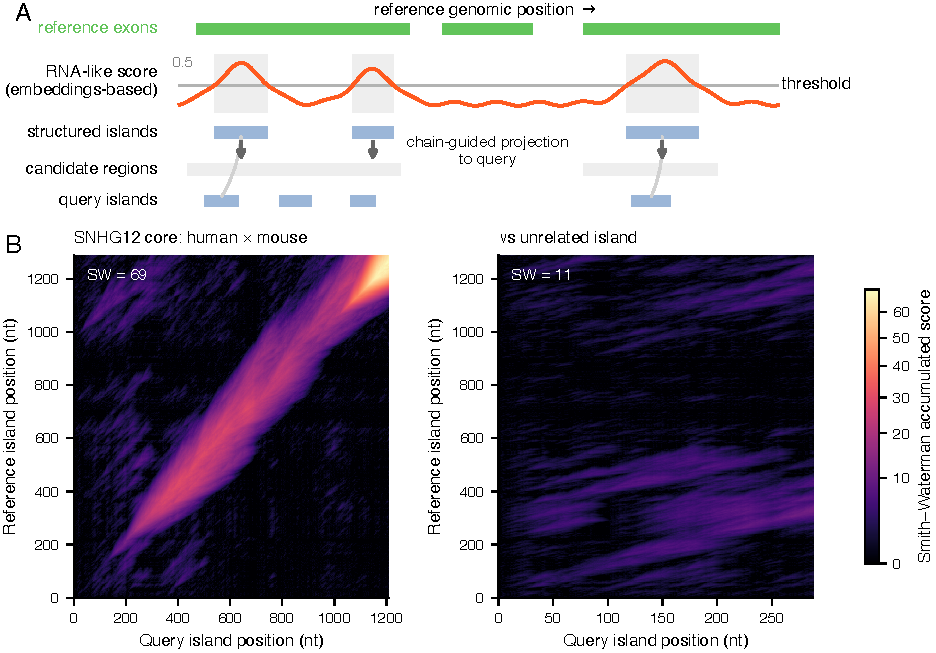
\includegraphics[width=\linewidth]{fig3_islands.pdf}
  \caption{Identification and matching of localized ncRNA subregions using
  embedding-based similarity. \textbf{(A)} Schematic: an embedding-based detector
  score along a reference transcript is thresholded to define localized subregions
  (``islands''); islands are projected via genome alignment chains to candidate
  query regions, where corresponding islands are detected independently.
  \textbf{(B)} Island
  matching for a recurrent lncRNA region (SNHG12, human hg38 chr1 $\times$ mouse
  mm39 chr4). Each island is embedded once; the per-token cosine dotplot is aligned
  by Smith--Waterman, shown here as the accumulated-score matrix. The conserved
  matched region forms a single coherent diagonal ridge (embedding-SW alignment score $69$), whereas the same
  human island against an unrelated mouse island yields no coherent alignment
  (embedding-SW alignment score $11$).}
  \label{fig:islands}
\end{figure}

\subsection{Evaluation metrics}
\label{sec:eval}

Evaluation is based on agreement with existing annotations and is used as an
approximate proxy for ground truth. Because ncRNA annotations are incomplete and
heterogeneous across species, the reported metrics should be interpreted as
measures of annotation agreement rather than direct estimates of biological
accuracy.

\subsubsection{Short ncRNA evaluation}

For short ncRNAs, evaluation is performed at the locus level against annotated
transcripts using three distinct criteria:
\begin{itemize}
    \item \emph{any-overlap rate}: the fraction of predictions intersecting an
    annotated ncRNA exon by at least $1$\,nt;
    \item \emph{$50\%$ prediction coverage}: the fraction for which the maximum
    exonic intersection with an annotated transcript, divided by the
    predicted-locus length, is at least $50\%$;
    \item \emph{near-complete prediction coverage}: the fraction satisfying the
    same one-directional criterion at $99\%$.
\end{itemize}

We separately report workflow coverage across the full set of eligible reference
loci: the number of non-protein-coding union loci satisfying the short-branch
geometry, the number assigned at least one chain-projected query candidate, and
the number producing a refined prediction. These counts describe processing
yield rather than biological recall. Estimating recall would require a linked
set of eligible human loci with established mouse counterparts; query-side
interval overlap alone does not establish such a relationship.

As a conservative proxy, we also define a \emph{named-counterpart} set consisting
of eligible human loci whose gene name occurs exactly, ignoring case, in the
mouse GENCODE annotation. A locus is counted as recovered when its final
prediction overlaps an exon of the same-named mouse gene. This criterion is
enriched for established, consistently named RNA families and should not be
interpreted as a general genome-wide recall estimate.

\subsubsection{Evaluation of localized-subregion predictions}

For loci processed by the localized-subregion workflow, evaluation is performed
at both the locus and subregion levels. A reference locus is considered supported
when at least one predicted query subregion overlaps an annotated ncRNA exon. At
the subregion level, a matched island is considered supported when it overlaps an
annotated ncRNA exon in the query genome.

We report the fraction of supported loci, the fraction of matched islands
overlapping annotated exons, the distribution of exonic overlap proportions, and
the number of matched islands per locus. For multi-species analyses, recurrence
is summarized by the number of query genomes in which a reference subregion has
an accepted match.

To examine the relationship between embedding-based match strength and annotation
support, predictions are stratified by score. We report annotation-overlap rates
across score bins and compare score distributions between overlapping and
non-overlapping predictions. Because the scores are not globally calibrated,
these analyses characterize an empirical association with annotation support
rather than a formal measure of prediction confidence.

Predictions outside annotated regions may represent either false positives or
currently unannotated ncRNAs
\citep{hezroniPrinciplesLongNoncoding2015,
    mattickLongNoncodingRNAs2023,
    perteaCHESSNewHuman2018}.
Annotation completeness varies across species, and ncRNA boundaries are often
imprecise. Unlike protein-coding ORFs, many ncRNAs lack sharply defined,
independently verifiable functional boundaries. Overlap-based evaluation should
therefore be interpreted as an annotation-agreement measure rather than as a
precise benchmark of biological accuracy or boundary recovery.

\subsection{Recurrent-core aggregation and coding proximity}

Reference islands obtained from different species comparisons are assigned to the
same recurrent core when their human reference intervals overlap within the same
gene. For each core and query species, only the accepted match with the lowest
embedding-SW distance is retained.

A query species is counted as supporting a core when it contains an accepted
island match. Because accepted matches already satisfy the pipeline threshold
$d \leq 0.10$, the broad recurrent set is defined by support in at least 17 of
19 query species and by a mean reference-island length of at least 120\,bp. This
length is calculated across the retained species-specific human reference-island
intervals contributing to the core, with at most one interval per query species;
it is distinct from the total span of the aggregated core.

For sensitivity analyses, recurrence was recalculated using stricter
per-species distance thresholds of $d \leq 0.05$, $0.04$, $0.03$, $0.02$, and
$0.01$, while fixing the required species count at 17. We also varied the species
quorum while fixing the per-species threshold at $d \leq 0.02$.

To characterize coding proximity, human lncRNA gene spans were compared with
protein-coding gene spans. Direct overlaps were classified by strand as sense,
antisense, or both. Non-overlapping lncRNA loci within 5\,kb of a protein-coding
gene were classified as near coding, and all remaining loci as intergenic. These
categories describe genomic proximity only and do not imply transcriptional or
functional relationships.

\subsection{Exploratory ViennaRNA structure comparison}

The exact human--mouse intervals for the three short-ncRNA examples in
Figure~\ref{fig:cases} and the accepted MALAT1 recurrent-core matches R5, R4, R3,
and R2 were analyzed with ViennaRNA 2.7.2
\citep{lorenzViennaRNAPackage2011}. The similar-length short-ncRNA intervals were
folded as complete sequences. For each MALAT1 core, length-matched windows were
defined from the aligned span and expanded symmetrically by 20 or 40\,nt.

Global partition-function folding and RNAplfold were applied. Human and mouse
sequences were aligned using affine-gap nucleotide Smith--Waterman, and the
resulting alignment was used to place both base-pair probability matrices in a
shared coordinate system. Structural agreement was then summarized using a
column-exact weighted Jaccard score and a $\pm2$-column tolerance-aware weighted
overlap with one-to-one matching.

These metrics are exploratory descriptive measures and have not been validated as
general structure-similarity scores. Full per-window and per-method results are
provided in Supplementary Figures S1--S7, Supplementary Table S1, and the source
TSV files.

\subsection{Implementation details}
\label{sec:impl}

Embeddings are computed with RiNALMo and projected using the two task-specific PCA
transformations described in Section~\ref{sec:embeddings}: $1280 \to 16$ for
position-level matching and $1280 \to 64$ for localized-subregion detection.
Compact-locus sequences are embedded separately for each candidate window,
whereas complete reference and query islands are embedded to obtain the per-token
matrices used by the local matcher.

Embedding inference is performed on GPU using batched execution. MMD computation,
cosine-similarity alignment, match assignment, and downstream filtering are
performed on CPU. \curia{} is implemented as a staged task pipeline that separates
embedding inference from subsequent analysis. Sequence windows are processed by a
shared GPU worker using micro-batching, and intermediate representations are
persisted for reuse by later stages and across query-genome runs.

RiNALMo inference uses PyTorch memory-efficient scaled-dot-product attention.
Pipeline outputs are written in tabular and BED formats. Embedding-model versions,
PCA transformations, detector parameters, and matching thresholds are stored as
versioned pipeline artifacts.

\section{Results}
\label{sec:results}

\subsection{Benchmark setup}
\curia{} was evaluated on a panel of 19 mammalian genomes, using human (hg38) as
the reference and the others as queries, spanning primates through the marsupial
outgroups: rhesus macaque (rheMac10), mouse (mm39), rat (rn7), rabbit (HLoryCun3),
cow (bosTau9), pig (susScr11), Bryde's whale (HLbalEde1), dromedary (HLcamDro2),
horse (equCab3), cat (felCat9), dog (canFam5), pangolin (HLmanJav2), flying fox
(HLpteVam2), hedgehog (eriEur2), armadillo (dasNov3), Asian elephant (HLeleMax1),
and three marsupials --- gray opossum (monDom5), Virginia opossum (HLdidVir1), and
tammar wallaby (HLnotEug3). Genome assemblies
were obtained from NCBI \citep{sayersDatabaseResourcesNational2022} and the UCSC
Genome Browser \citep{kentHumanGenomeBrowser2002}. Due to variability in
annotation quality across species, high-quality ncRNA annotations were used only
for human (GENCODE V48) and mouse (GENCODE VM37)
\citep{harrowGENCODEReferenceHuman2012}, while other species were analyzed without
relying on their native annotations. Human and mouse contain on the order of
${\sim}20{,}000$ annotated ncRNA transcripts, spanning both well-supported
elements (e.g., tRNAs, rRNAs, selected snoRNAs) and less-characterized transcripts,
particularly among lncRNAs. Evaluation was performed at both the locus level (for
short ncRNAs and lncRNA loci) and the substructure level (for island matches),
following the criteria defined in Section~\ref{sec:eval}.

\subsection{Overall performance}
We first evaluated agreement between predicted loci and existing annotations. In
the human-to-mouse evaluation (mouse being the query for which a comprehensive
reference annotation is available), among 2{,}994 predicted short ncRNA loci
52.4\% show any overlap with an annotated exon ($\geq 1$\,nt; any-overlap rate),
46.5\% meet a reciprocal-overlap recovery criterion (predicted locus covering
$\geq 50\%$ of the annotated transcript), and 26.0\% meet near-complete boundary
recovery ($\geq 99\%$ overlap). Among any-overlap predictions, the median overlap
is 98.9\% (mean 86.8\%), indicating that matched loci are typically well
localized and consistent with annotated boundaries.

These results suggest that matched loci are generally well localized when
annotation support is present. The substantial fraction of predictions without
annotation overlap is consistent with a combination of annotation incompleteness,
projection errors, and potential false positives. Notably, many non-overlapping
predictions retain strong syntenic support, suggesting that some may correspond to
unannotated or weakly annotated ncRNA loci.

\subsection{Short ncRNA performance and score behavior}
% RiNALMo human-mouse numbers (analysis/pair_numbers.py + compute_fig4_data.py).
We evaluated similarity between matched short ncRNA loci using MMD in embedding
space. For the human--mouse pair (2{,}994 loci), the MMD distribution is skewed
toward low values (median 0.142; Fig.~\ref{fig:mmd}A), with a substantial fraction
of near-zero values (32.5\% below 0.05), indicating consistent embedding
representations between matched reference and query loci.

Stratification by biotype reveals clear differences (Fig.~\ref{fig:mmd}C).
snoRNAs and tRNAs exhibit the lowest MMD values (median $\approx 0$), consistent
with their strong, well-characterized structural conservation
\citep{chanTRNAscanSE20Improved2021}. miRNAs and lncRNAs occupy an intermediate
range, whereas snRNAs, misc\_RNAs, and rRNA-derived loci show higher and broader
distributions, likely reflecting copy number, sequence divergence, and genomic
context.

MMD is strongly associated with annotation overlap. Predictions with low MMD
values ($\lesssim 0.1$) show high any-overlap rates with annotated loci
(${\sim}88\%$),
whereas higher MMD values show reduced overlap and increased dispersion.
Predictions with MMD $> 0.2$ rarely overlap annotations and are enriched for
ambiguous cases. Consistent with this, loci overlapping annotations are enriched
at low MMD values, while non-overlapping predictions are shifted toward higher
values (Fig.~\ref{fig:mmd}B), supporting the interpretation of MMD as a continuous
empirical measure of correspondence confidence.

Notably, a subset of high-confidence predictions (MMD $\approx 0$) does not
overlap existing annotations despite strong syntenic support, suggesting that
annotation incompleteness contributes to the observed gap.

To assess whether embedding-based similarity merely recapitulates sequence
conservation, we compared MMD to pairwise sequence identity for matched short
ncRNA loci. The two measures were strongly anticorrelated (Pearson $r = -0.80$;
Spearman $\rho = -0.85$; $n = 1{,}500$ sampled loci). However, this relationship is not
deterministic: at intermediate sequence identity ($\approx 40$--$60\%$), MMD
values span a broad range, indicating that embedding similarity is related to,
but not fully determined by, pairwise sequence identity in this regime.

\begin{figure}[t]
  \centering
  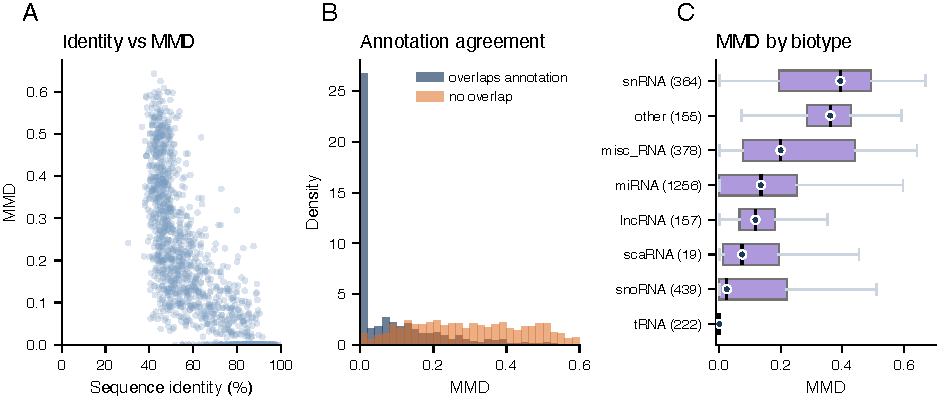
\includegraphics[width=\linewidth]{fig4_mmd.pdf}
  \caption{Behavior of embedding-based similarity (MMD) across short ncRNA loci
  for the human--mouse pair. \textbf{(A)} Sequence identity versus MMD for matched
  loci (strongly anticorrelated). \textbf{(B)} MMD distributions for loci that do
  versus do not overlap mouse annotation: annotation-overlapping loci concentrate
  at low MMD, non-overlapping loci shift higher. \textbf{(C)} MMD distribution by
  ncRNA biotype, ordered by median.}
  \label{fig:mmd}
\end{figure}

\subsection{Structural conservation analysis (``islands'')}
% Island match metric is cosine-Smith-Waterman distance d = 1/(1+score), not MMD.
We analyzed localized subregions (``islands'') within lncRNAs to assess
cross-species correspondence beyond the locus level. Islands are matched at
nucleotide resolution by Smith--Waterman alignment over the per-token cosine
similarity dotplot, and match quality is reported as a cosine-SW distance
$d = 1/(1+\text{score})$ (lower is better; Section~\ref{sec:islandalign}). Island
detection reveals that embedding-supported signal is sparse and localized. Most
lncRNAs contain a small number of discrete islands rather than uniform signal
across the full transcript (Fig.~\ref{fig:cores}A), indicating that the strongest
cross-species signal is concentrated in compact subregions. Across loci, islands
were detected in approximately 54\% of lncRNAs, with a median of 2 islands per
transcript.

To assess cross-species correspondence, we evaluated matches between reference and
query islands. At the gene level, 96.9\% of islanded lncRNAs exhibit at least one
cross-species match in at least one query species, indicating that detectable
correspondence is widespread but rarely spans entire transcripts. About half of
matched islands (50.1\%) overlap annotated ncRNA regions in the query genome, and
28.6\% show $\geq 50\%$ exonic overlap, suggesting that a substantial fraction of
candidate elements are not captured by current annotation resources.

Together, these observations support a modular pattern of cross-species
correspondence, with signal concentrated in discrete localized regions rather than
uniformly distributed across entire transcripts
\citep{hezroniPrinciplesLongNoncoding2015,rivasEvolutionaryConservationRNA2021,ulitskyEvolutionRescueUsing2016,mattickLongNoncodingRNAs2023,quinnUniqueFeaturesLong2016}.
This interpretation is broadly consistent with observations from well-characterized
lncRNAs such as NEAT1, XIST, and MALAT1, in which localized domains have been
linked to distinct architectural, spreading, or stability-related functions
\citep{wiluszTripleHelixStabilizes2012,yamazakiFunctionalDomainsNEAT12018,engreitzXistLncRNAExploits2013}.

\subsubsection{Multi-species conserved cores}
Here, ``conserved cores'' refers operationally to islands showing recurrent
high-confidence matches across multiple species within syntenically projected
loci. We observe a subset of islands that exhibit reproducible cross-species
matches (Fig.~\ref{fig:cores}B--C), with increasing divergence at greater
phylogenetic distance. Across all detected cores, 87\% are recovered in at least
two species, 67\% in five or more species, and approximately 2\% are consistently
detected across all 19 species, including the marsupial outgroups (opossums and
wallaby).

In contrast to locus-level overlap, which is often incomplete or ambiguous, these
cores exhibit stable cross-species correspondence at the level of localized
embedding similarity. To assess whether such matches could arise from selecting
the best of many candidate positions within a syntenic window, we compared each
matched query island against same-length windows tiled across its own projected
syntenic locus (a within-locus positional null; representative genome pairs). The
assigned position was the best-scoring one far more often than expected by chance,
and its advantage over the alternatives \emph{increased} with the number of
independent same-locus positions rather than collapsing toward chance, indicating
that recurrent cores are unlikely to be artifacts of a best-of-many maximum within
syntenic regions.

\subsection{Candidate conserved regions absent from current annotations}
After excluding regions overlapping or proximal to protein-coding genes, we
identify approximately 230 candidate intergenic loci potentially corresponding to
conserved ncRNA elements, exhibiting consistent embedding-space similarity across
$\geq 18$ of the 19 species (of 1{,}107 conserved-core lncRNA loci in total). The
full set of loci (all conservation categories) is provided as a supplementary
table in the repository:
\url{https://github.com/kirilenkobm/CURIA_pipeline/blob/master/paper/lncRNAs_with_conserved_cores.tsv}.
These loci
represent candidate elements and may include false positives despite filtering.
The persistence of these loci after filtering suggests that the observed signal is
unlikely to be primarily driven by coding-associated conservation, although
residual confounding cannot be excluded.

\subsection{Case studies}
To illustrate the behavior of \curia{}, we examined individual loci
(Fig.~\ref{fig:cases}). Projection of human SNORD57 to mouse identifies a nearly
exact match overlapping annotated Snord57, demonstrating precise localization
under strong structural conservation. Projection of human RNU6-7 intersects an
annotated mouse locus (Gm24859), indicating recovery of a corresponding genomic
region despite ambiguous or incomplete annotation. Projection of human vault RNA
(ENSG00000199990) identifies a corresponding locus overlapping mouse Vaultrc5; the
matched region differs in length from the human transcript, yet \curia{} localizes
the most similar segment within the syntenic region.

\begin{figure}[t]
  \centering
  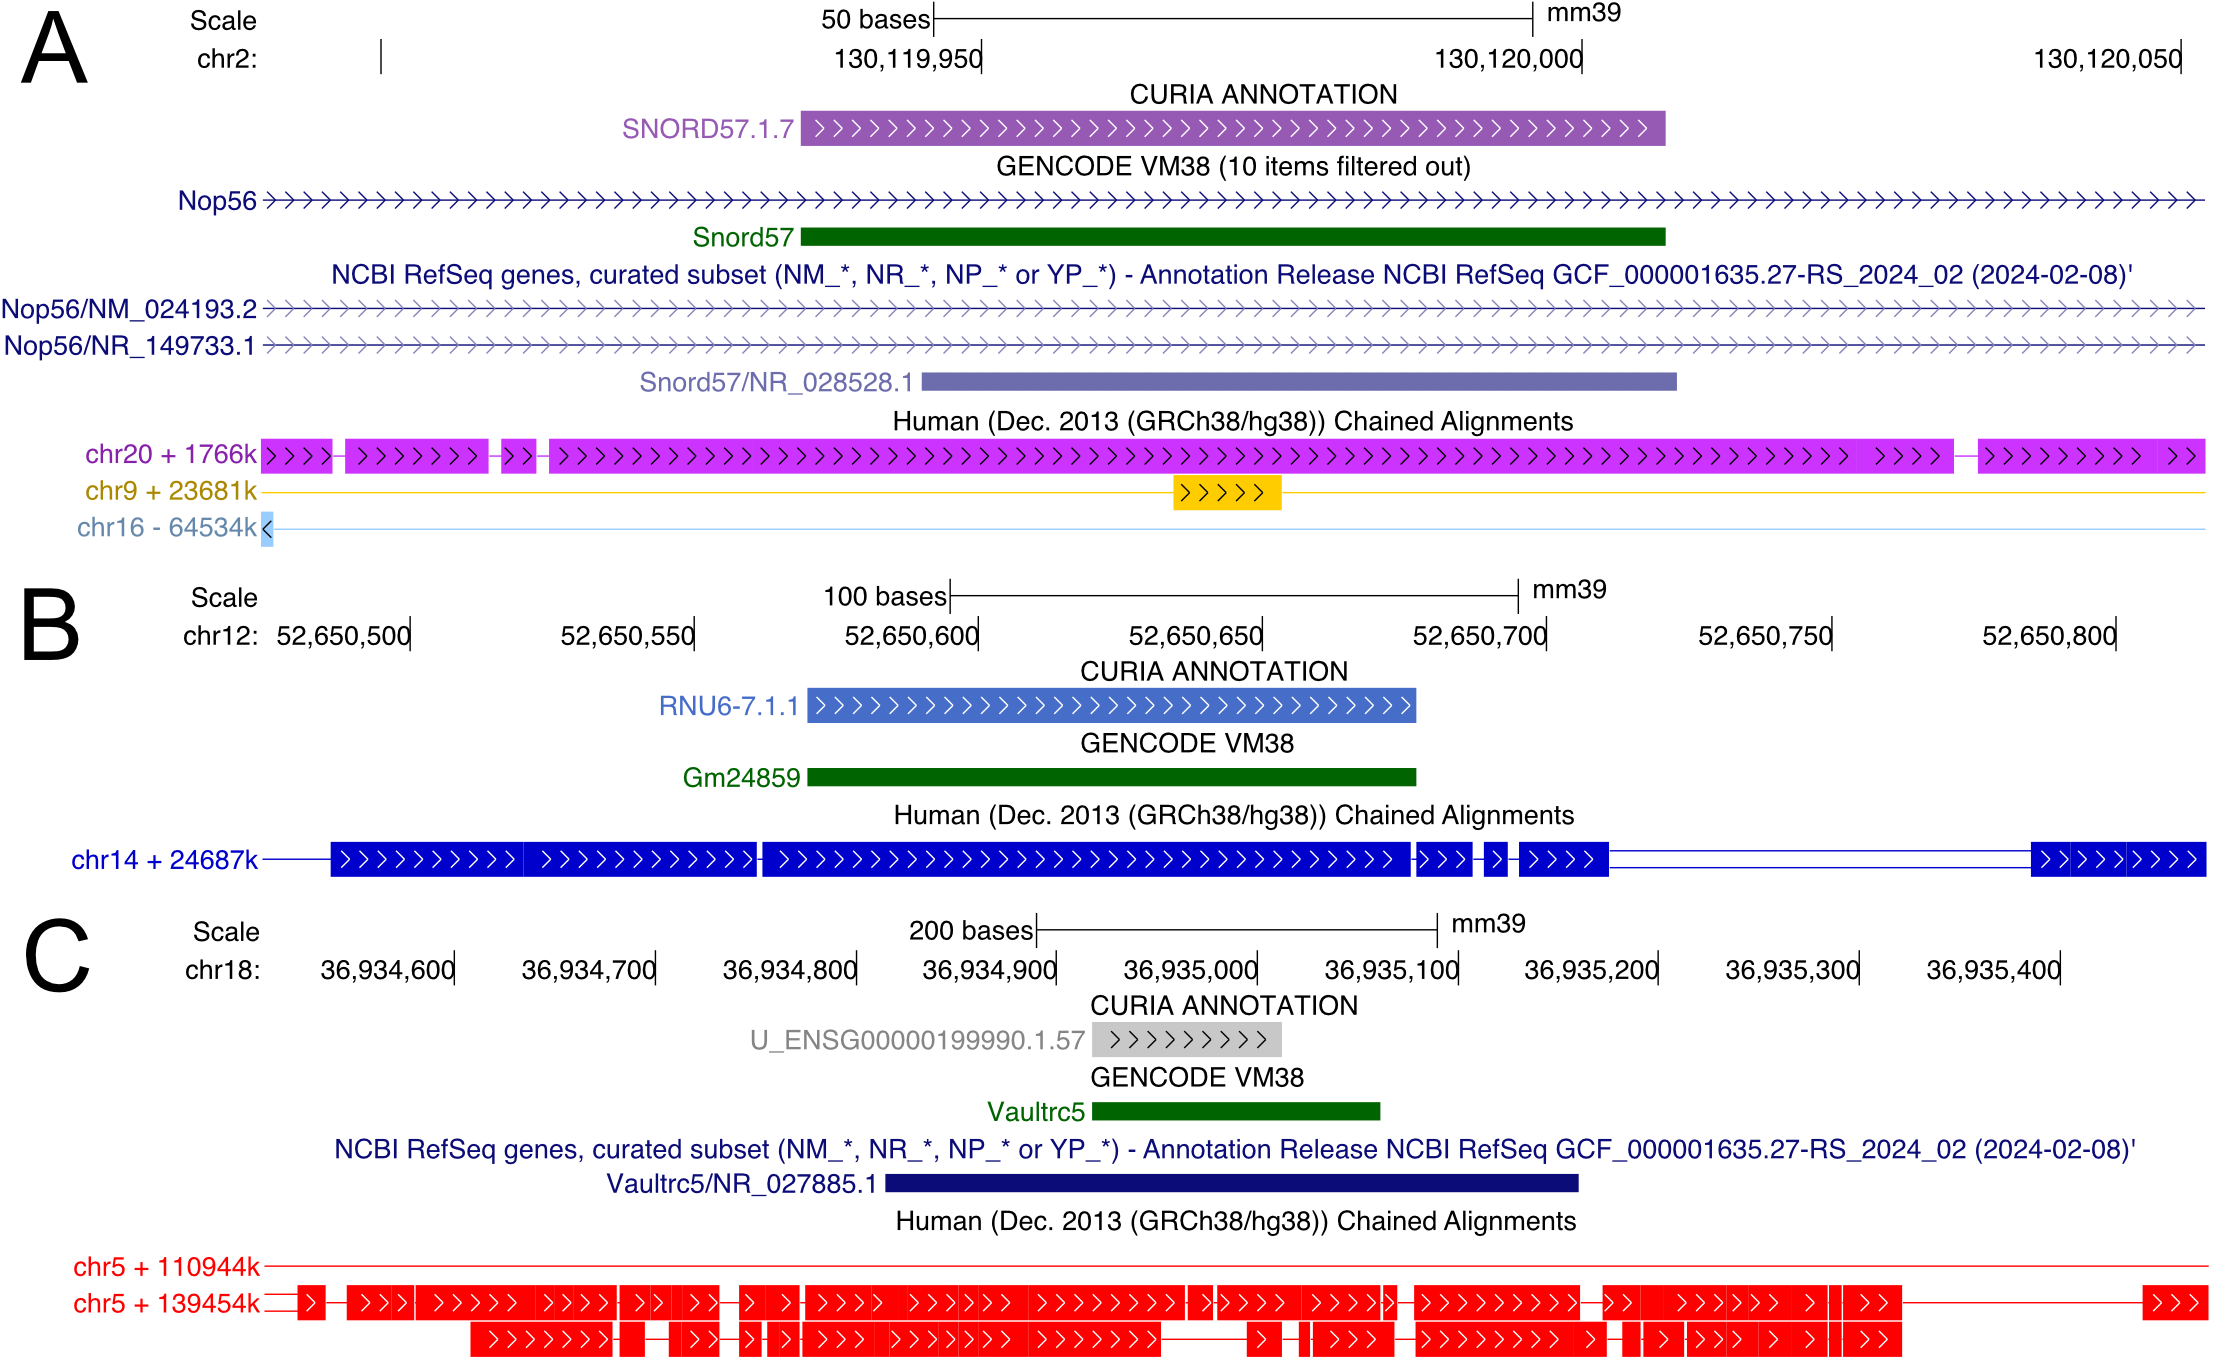
\includegraphics[width=\linewidth]{fig5_cases.png}
  \caption{Recovery of short ncRNA loci across species using \curia{}. Genome
  browser snapshots (UCSC) illustrating representative examples of short ncRNA
  projection from human (hg38) to mouse (mm39): SNORD57 (exact match), RNU6-7
  (recovery under incomplete annotation), and vault RNA (length divergence,
  partial correspondence).}
  \label{fig:cases}
\end{figure}

\begin{figure}[t]
  \centering
  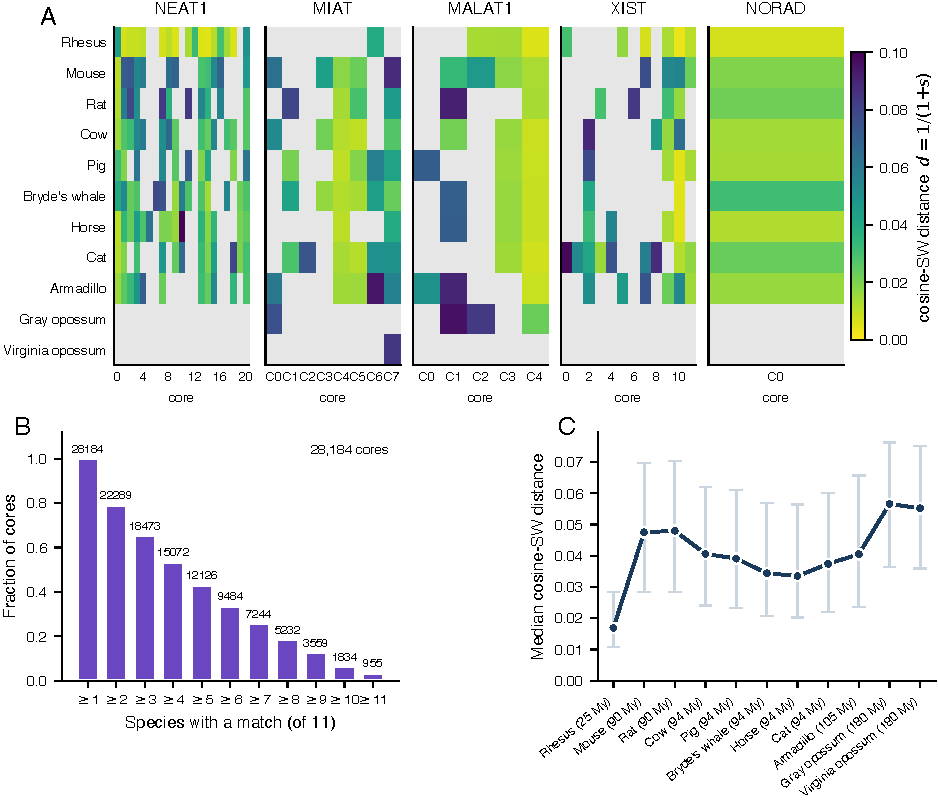
\includegraphics[width=\linewidth]{fig6_cores.pdf}
  \caption{Modular and heterogeneous cross-species correspondence of lncRNA cores.
  \textbf{(A)} Cross-species matching of core regions for representative lncRNAs
  (NEAT1, MIAT, MALAT1, XIST, NORAD); rows are species, columns are reference cores ordered along
  the transcript, color indicates match distance (cosine-SW distance $d=1/(1+s)$). \textbf{(B)} Distribution of
  core reproducibility across species. \textbf{(C)} Median island-level match
  distance across species, increasing with phylogenetic distance.}
  \label{fig:cores}
\end{figure}

\subsection{Error analysis}
The dominant failure modes arise from limitations in projection, annotation, and
signal strength. Chain-based projection defines the search space and acts as a
hard constraint: if the corresponding region is not captured by genome alignments,
it cannot be recovered. Incomplete and imprecise reference annotations further
limit recoverable signal, particularly for lncRNAs. A substantial fraction of loci
exhibit weak or diffuse embedding signal, producing no detectable islands or only
fragmented matches. Overall, most observed failures are associated with missing or
ambiguous signal and projection constraints, rather than instability of the
downstream matching procedure.

\subsection{Runtime and scalability}
% TODO(authors): confirm the exact GPU/CPU used for the reported panel (runs
% spanned more than one machine). Wall-time range below is measured from the 19
% completed run logs: min 1h09m, median ~2h27m, max 4h18m.
We evaluated \curia{} on the 19 genome-pair panel. On a single GPU, a full
genome-pair run completes in roughly one to four hours (median ${\sim}2.5$\,h
across the 19 pairs), scaling approximately linearly with annotation size.
Embedding inference is performed on GPU with batched execution, while downstream
matching and alignment are CPU-bound; both reference and query island detection
are restricted to syntenically projected regions, substantially reducing the
effective search space.

\section{Discussion}
\label{sec:discussion}

\curia{} should be viewed primarily as a proof of concept demonstrating that
synteny-constrained embedding comparison yields interpretable cross-species signal
for ncRNA correspondence at genome scale, rather than as a finished annotation
framework optimized for exhaustive sensitivity or production use. Within this
framing, several key observations emerge.

\subsection{Key findings}
We show that cross-species ncRNA correspondence can be recovered at genome scale
using a combination of syntenic constraints and embedding-based similarity. This
enables identification of candidate corresponding loci even in the absence of
strong sequence conservation. For short ncRNAs, correspondence is typically well
localized when supported by annotation, and embedding-based similarity provides a
consistent empirical measure of match confidence. For long ncRNAs, correspondence
is frequently partial and localized, with signal concentrated in discrete
subregions rather than spanning full transcripts. Together, these results support
a model in which cross-species ncRNA correspondence is heterogeneous and modular,
and can be captured using localized comparison in embedding space.

\subsection{Comparison to existing methods}
Existing approaches provide complementary capabilities for ncRNA detection and
structural comparison but do not directly address genome-scale correspondence.
Covariance models require curated family models, while explicit structure
alignment compares supplied RNA sequences rather than locating corresponding
elements from genome and reference annotation alone. Genome-wide scanning
approaches identify candidate RNA elements but do not establish explicit
cross-species correspondence. Methods specifically targeting
lncRNA homology are most directly comparable: slncky infers lncRNA orthologs from
whole-genome alignments using sequence-level conservation signatures, and lncHOME
groups lncRNAs into families based on conserved genomic position combined with
patterns of RNA-binding-protein motifs
\citep{chenEvolutionaryAnalysisMammals2016,huangComputationalPredictionExperimental2024}.
Both rely on primary-sequence or motif-level signals to define homology. In
contrast, \curia{} does not require strong end-to-end sequence conservation
within the ncRNA itself. It combines whole-genome-alignment-derived syntenic
constraints with embedding-based similarity, so
correspondence can be proposed for loci whose primary sequence has diverged beyond
the reach of alignment- or motif-based comparison, without requiring curated
families or explicit structural alignment.

\subsection{Biological implications}
Beyond the modular correspondence pattern noted above, two observations bear on
interpretation. For long ncRNAs, correspondence frequently concentrates in compact
subregions while the surrounding transcript context shows weak or no detectable
similarity. And for short ncRNAs, although embedding-based similarity is strongly
associated with sequence identity, the relationship is not uniform: at intermediate
sequence identity ($\approx 40$--$60\%$), substantial variability is observed,
indicating that loci with comparable sequence similarity can exhibit markedly
different embedding-based similarity.

The island-based representation provides a practical way to capture this behavior:
recurrent embedding-supported islands define candidate corresponding regions, while
intervening regions appear less constrained. Correspondence patterns also vary
across RNA classes: compact RNAs such as tRNAs and snoRNAs show strong and
consistent signal, whereas long ncRNAs more often exhibit partial or fragmented
correspondence
\citep{hezroniPrinciplesLongNoncoding2015,ulitskyEvolutionRescueUsing2016,mattickLongNoncodingRNAs2023}.
Together, these observations support a model in which recurrent candidate elements
are embedded within broader, weakly constrained transcript contexts, emphasizing
the importance of localized comparison in cross-species ncRNA analysis.

\subsection{Limitations}
This study has several limitations related to data availability, modeling
assumptions, and evaluation. First, the lack of reliable ground truth for
cross-species ncRNA correspondence remains a major challenge; existing annotations
are incomplete and heterogeneous across species, and transcript boundaries---particularly
for lncRNAs---are often ambiguous. As a result, evaluation based on
annotation overlap provides only an approximate and conservative estimate of
performance.

Second, \curia{} depends on the availability and quality of genome alignment
chains. Because the search space is restricted to aligned regions, correspondence
cannot be recovered outside chain coverage, and errors or fragmentation in
alignments propagate directly to downstream predictions. In addition, the
candidate-region classification step is adapted from protein-coding gene
projection and may not fully capture the diversity of ncRNA correspondence
patterns.

Third, the method relies on embedding representations derived from RNA foundation
models. Although RiNALMo \citep{penicRiNALMoGeneralpurposeRNA2025} provides a
practical representation, it may not capture all relevant structural features.
The island detector was trained on known compact structured ncRNAs against genomic
background. A genuine lncRNA core whose embedding pattern lies outside that
positive class may therefore be classified as background and never reach the
matcher. Repository held-out-family analyses show broad generalization across
structured-RNA families but substantially weaker recall for lncRNA, consistent
with this failure mode. In particular, \curia{} is primarily sensitive to localized
signal in embedding space and does not model long-range interactions or global RNA
architecture. Because it assumes approximate collinearity within candidate regions
and scores local similarity, it does not capture rearrangements of structured
elements; loci lacking localized embedding signal are unlikely to yield detectable
correspondence.

Fourth, \curia{} does not establish transcriptional activity or molecular
function; predicted regions represent candidate corresponding elements and require
additional transcriptomic or experimental validation. Annotation-discordant calls
have several competing interpretations---missing or imprecise query annotation,
projection or assembly error, correspondence to a different nearby element, or a
false-positive match---which cannot be resolved from interval overlap alone. We
therefore report annotation agreement rather than treating it as either precision
or recall.

Finally, \curia{} does not explicitly distinguish between shared evolutionary
origin and convergent similarity at the level of embedding space. While synteny
strongly biases predictions toward corresponding loci with shared ancestry,
embedding similarity may also capture convergent structural features or recurrent
local motifs. Accordingly, high-confidence matches should be interpreted as
candidate corresponding elements supported by both synteny and embedding
similarity, rather than definitive evidence of shared evolutionary origin.

\subsection{Embedding-based similarity and interpretability}
Embedding representations used in \curia{} are derived from RNA foundation models
trained on large collections of RNA sequences without explicit structural
supervision
\citep{chenInterpretableRNAFoundation2022,akiyamaInformativeRNABase2022,vahabAdvancingNoncodingRNA2025}.
Prior work has shown that such models encode representations associated with RNA
secondary structure and related functional properties, and can support downstream
structure prediction tasks \citep{shenAccurateRNA3D2024}. In this context,
embedding similarity provides an implicit measure of correspondence that is not
tied directly to primary-sequence identity. Empirically, match scores form a
continuous scale separating high-confidence matches from background signal. This
interpretation is broadly consistent with observations from protein language
models, where representations learned from sequence alone organize according to
structural and functional properties \citep{rivesBiologicalStructureFunction2021}.

\subsection{Future directions}
The most informative next step is biological interpretation of the recovered
cores. Predicted elements can be prioritized for secondary-structure analysis,
candidate interaction surfaces and binding partners, transcriptomic support, and
targeted validation. Comparing the number, order, and divergence of cores across
species may reveal how lncRNAs gain, lose, or rearrange functional modules and may
identify recurrent mechanisms that are obscured at whole-transcript scale.

Methodologically, combining core matches across species in a phylogenetic model
could distinguish conserved ancestry from recurrent similarity and reduce the
impact of a single poor assembly or chain set. Multi-scale representations may
also connect locally detectable cores to longer-range RNA architecture.

\section{Data and code availability}
\label{sec:availability}

The \curia{} pipeline is available at the project repository:
\url{https://github.com/kirilenkobm/CURIA_pipeline}. Preprocessed reference
annotation files used in this study are provided in the repository under
\texttt{input\_data/reference\_annotation/}. The recurrent-core tables described
in Section~\ref{sec:results} are included in the repository under
\texttt{paper/recurrent\_core\_tables/}. This directory contains gene-level,
core-level, and core-by-assembly match tables, distance and quorum sensitivity
tables, and a README defining coordinates, identifiers, acceptance criteria, and
derived fields. The historical gene-level summary remains available alongside
the package. The per-species predictions
and analysis tables underlying the preprint are provided under
\texttt{preprint\_results/}. The exploratory ViennaRNA supplement is provided as
\texttt{paper/supplementary/vienna\_structure\_supplementary.pdf}, containing
Supplementary Figures S1--S7 and Supplementary Table S1. Its machine-readable
per-window results, source data, and diagnostic plots are provided under
\texttt{analysis/vienna\_structure\_examples/}, including
\texttt{malat1\_windows.tsv}. Genome assemblies (2bit
format) were obtained from NCBI \citep{sayersDatabaseResourcesNational2022} and
UCSC Genome Browser \citep{kentHumanGenomeBrowser2002} resources. Genome alignment
chains were obtained from the TOGA project (Hiller lab)
\citep{kirilenkoIntegratingGeneAnnotation2023}:
\url{https://genome.senckenberg.de/download/TOGA}. All external datasets are
publicly available, and links to the exact sources are provided in the repository.


\bibliographystyle{unsrtnatetal}  % unsrtnat + author truncation (see paper/README)
\bibliography{CURIA_Preprint}

\end{document}
